\section{Simulation}\label{sec:analysis.simulation}
There are certain kinematic regions of \abbr{CLAS} in which physics events are not being recorded properly i.e.~the area dividing each sector in \abbr{CLAS}. Furthermore each sector in \abbr{CLAS} is asymmetric in the acceptance of events due to subsystem inefficiencies such as inoperable \abbr{DC} wires, \abbr{PMT} inefficiencies, dead scintillator strips the the \abbr{TOF} and \abbr{ST} subsystems. When a triggered event is recorded and reconstructed these asymmetric inefficiencies factors are reflected and must be carefully understood because these factors are properties of the \abbr{CLAS} detector and independent of any physics that occurred. To properly understand the detector effects on the data, \abbr{CLAS} utilizes a \abbr{GEANT} simulation package know as \abbr{GSIM}. To prepare an event for \abbr{GSIM} the program \abbr{GAMP2PART} converts a text file, containing the 4-momentum of the generated event, into a suitable file format for \abbr{GSIM}. \abbr{GSIM} then simulates the passage of these particles through the \abbr{CLAS} detector and generates the associated \abbr{ADC} and \abbr{TDC} information from detector hits. \abbr{GSIM} takes into account detector inefficiencies described in the \abbr{\texttt{CLAS\_CALDB\_RUNINDEX}}. The \abbr{CLAS\_CALDB\_RUNINDEX} is an array of information about each subsystem's inefficiency that was derived during the g12 calibration process. The \abbr{GSIM} simulated hits are then ``post-processed'' by smearing the \abbr{TDC} and \abbr{ADC} hits to imitate the observed resolution of the detector subsystems using the program \abbr{GPP} (\abbr{GSIM} post-processor). \abbr{GPP} also removes detector hits due to inefficient \abbr{DC} wires. The simulation output processed with \abbr{GPP} is then reconstructed with \texttt{a1c}, the same program used to reconstruct data events. The reconstructed simulation is subject to the same scrutiny as real data events, undergoing all the cuts (Sec.~\ref{sec:evnt}), corrections~\cite{g12note}, and kinematic fitting (Sec.~\ref{sec:analysis.fitting}), as the real data except for beam corrections~\cite{g12note}.
\subsection{Simulation Verification}\label{sec:analysis.accept.verify}
Part of understanding the simulation output is understanding how well the simulation mimics the real data. To investigate this, 26,000 real \epemT events were treated as generated events and inputted into the \\ \abbr{GAM2PART}$\to$\abbr{GSIM}$\to$\abbr{GPP}$\to$\texttt{a1c}
\\ chain. Of the 26,000 events, only 100 were successfully reconstructed through the simulation chain. The source of this low efficiency was due to the calibrations entries for the \abbr{CC} and \abbr{EC} in the \abbr{CLAS\_CALDB\_RUNINDEX} not having values in which would set the ``PEDESTAL'' values appropriately for simulation. The calibrations constants in the \abbr{CLAS\_CALDB\_RUNINDEX} were correct for data reconstruction, but not for simulation reconstruction of \epemT in the \abbr{CC} and \abbr{EC} subsystems. It was also discovered that the \abbr{CC} and \abbr{EC} subsystems should be simulated with ``RUN 10'' constants instead of the normal ``RUN 56855'' used by the g12 group. ``RUN 56855'' is a special run benchmarked to have the best calibrations and required to properly simulate the \abbr{ST}, \abbr{DC}, and \abbr{TOF} subsystems. To rectify this, a special \abbr{CLAS\_CALDB\_RUNINDEX} was created, changing ``RUN 10'' to have ``RUN 56855'' constants for all subsystems except the \abbr{CC} and \abbr{EC} subsystems which were kept at ``RUN 10'' constants. Inputting the 26,000 real \epemT events into the simulation chain using the \abbr{CLAS\_CALDB\_RUNINDEX} \emph{RunIndexg12\_mk} outputted $\approx$~24,700 \epemT reconstructed events, i.e. $\approx$~95~\% efficiency.

The missing 5~\% was a result of ``time-based'' and ``hit-based'' tracking failures. The events that failed ``hit-based'' tracking contributes a 3.75~\% overall event inefficiency. The cause of the ``hit-based'' failure was never determined, but it was thought to have also occurred in the cooking of the data. Therefore since it did occur in the data reconstruction, this was considered to cancel the inefficiency of the simulation.

The ``time-based'' failure was due to a random bug in the processing of the \abbr{TDC} element information of \abbr{ST} (\abbr{STN0}) and the \abbr{ADC} element information of \abbr{ST} (\abbr{STN1}) raw data banks. The bug miscalculated the tracks sector exiting the \abbr{ST} even as the hit element of the \abbr{ST} matched that to the track in the \abbr{DC}. If the track failed due to this error, it usually passed ``time-based'' on the second or third pass of the ``time-based'' tracking if another particle passed ``time-based'' during the initial pass. The probability that a track failed initial ``time-based" tracking was $\approx$~.23\%. The probability that this failed event would pass ``time-based" tracking after another pass was $\approx99.78\%$. The average inefficiency for three charged track events for data was 0.0125\%

%This inefficiency depends on the distance the track is from the z-vertex position and can be seen in Fig.~\ref{fig:classt.ineffII}.
%\begin{figure}[h!]\begin{center}
%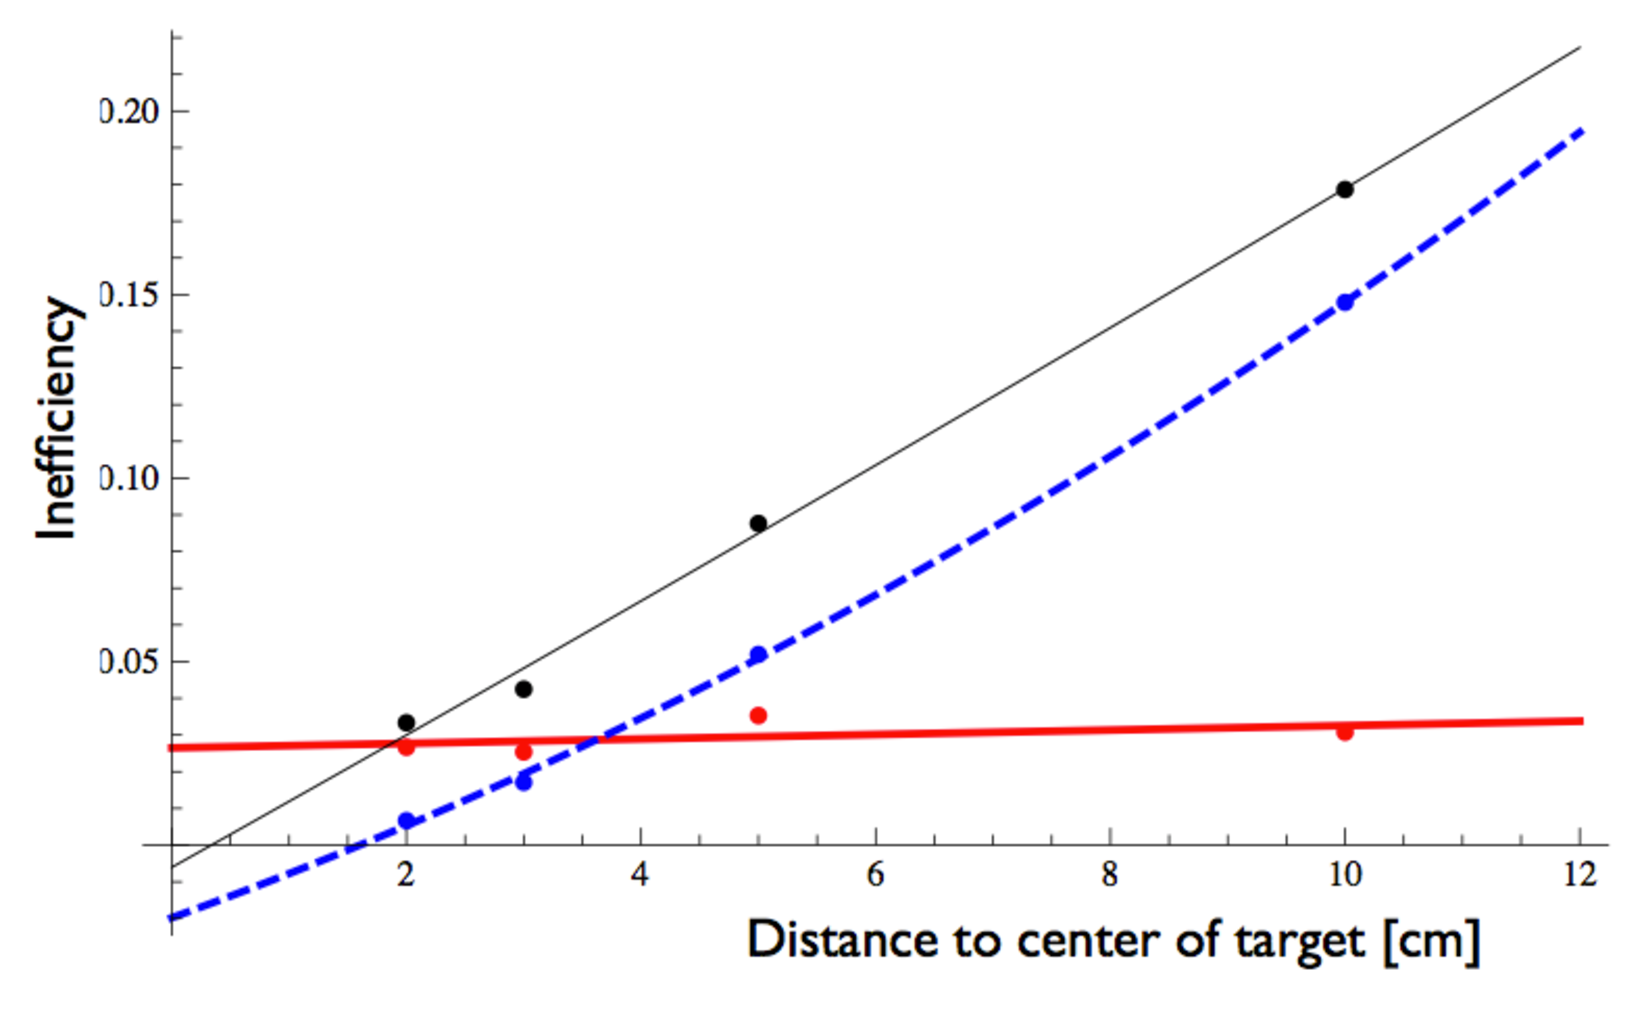
\includegraphics[width=0.8\figwidth,height=0.7\qfigheight]{\grpath/hall-b/st_issue_4_thesis.pdf}
%\caption[Start Counter Inefficiency]{\label{fig:classt.ineffII}{\coloronline}Plot showing the inefficiency of the start counter from data events, red-solid line is the inefficiency of reconstruction based solely on hit-based tracking, blue-dashed line is inefficiency of start counter, black-solid is combined. }
%\end{center}\end{figure}

\FloatBarrier
\subsection{PLUTO++ Event Generator}\label{sec:pluto}

Pluto~\cite{PLUTO} is a Monte-Carlo event generator designed for the study of hadronic interactions and heavy ion reactions in \abbr{HADES}, \abbr{FAIR} and upcoming \abbr{PANDA} collaborations. The versatility of Pluto enables its use as an event generator for photoproduction in \abbr{CLAS}. For hadronic interactions, Pluto can generate interactions from pion production threshold to intermediate energies of a few~GeV per nucleon. The entire software package is based on ROOT and uses ROOT's embedded C++ interpreter to control the generation of events. Programming event reaction can be set up with a few lines of ROOT macro code without detailed knowledge of programming. Some features in Pluto are, but not limited to;
\begin{itemize}
	\item Ability to generate events in phase space.
	\item Ability to generate events with a continuous bremsstrahlung photon beam.
	\item Ability to generate events weighted by a user defined $t$-slope.
	\item Ability to generate events weighted by a user defined cross-section.
	\begin{itemize}
		\item Total cross section can be inputted via functional form or histogram.
		\item Differential cross sections can be inputted via functional forms or histograms for specific beam energies up to 110 histograms relating to intervals of beam energy.
	\end{itemize}
	\item Ability to generate events that decay via already established physics parameters, i.e.~transition form factors.
	\item Ability to generate events that decay via modified established physics parameters.
	\item Ability to generate events with multiple production channels, weighted by user inputted cross-section probability.
	\item Ability to generate events with multiple decay channels, weighted by user inputted branching ratio.
	\item Ability to perform vertex smearing.
	\item Ability to create virtual detectors.
\end{itemize}

For the analysis presented in this work, Pluto was used in conjunction with known differential cross sections to verify simulation momentum smearing and tagger resolution, Sec.~\ref{sec:analysis.simsmear.verify}. Pluto was also utilized as a phase space generator in this analysis, to perform a ``tune'' on the kinematic fitter, Sec.~\ref{sec:analysis.fitting}, to calculate the acceptance corrections Sec.~\ref{sec:results.acceptance}, and to calculate the normalization Sec.~\ref{sec:results.normalization}.

\subsection{Simulating the Lepton Trigger}\label{sec:analysis.accept.trigger}
During the collection process, for an event to be written by the \abbr{DAQ} it must have passed at least one of the trigger ``bits" defined in Sec.~\ref{sec:clas.g12.conditions.data}. As discussed in Sec.~\ref{sec.data.trig.lepton}, the process of lepton triggering required a coincidence between the \abbr{EC} and the \abbr{CC} subsystems. This coincidence was established by using the voltage sum of the \abbr{CC} for a sector and the voltage sum of the \abbr{EC} for the same sector and comparing each sum to a preset threshold described in Table~\ref{tab:data.ecccthresh}. However when \abbr{GSIM} simulates tracks through the \abbr{CC} and \abbr{EC}, it does not account for the minimum voltage threshold that was required for data collection, moreover the simulation of the trigger must match the trigger efficiency discussed in Sec.~\ref{sec:analysis.trigger.verify}.

Simulation of the \abbr{CC} and \abbr{EC} trigger ``bit 6'', Sec.~\ref{sec.data.trig.lepton}, was performed by writing an algorithm that attempted to mimic the method in which triggered data was recorded. To accomplish this a modified function, written by Simeon McAleer from FSU, was written into the simulation reconstruction algorithm. The routine returned the sector and a boolean of 0 or 1 (pass or fail), that simulated the trigger based on the following criteria;
\begin{enumerate}\label{trig:sim.all}
	\item The sector with the highest EC summed energy over threshold. \label{trig:sim.ECtot} 
	\item The sector with the highest EC Inner Layer summed energy over threshold. \label{trig:sim.ECinner} 
	\item The sector with the highest CC summed energy over threshold. \label{trig:sim.CCtot} 
	\item All three above conditions must be in same sector.
\end{enumerate}
Thresholds as described in Table~\ref{tab:data.ecccthresh} are 80~mV, 60~mV and 20~mV for \abbr{EC} \emph{inner}, \abbr{EC}\emph{total} and CC respectively. The \abbr{CC} trigger threshold was applied to groups of eight \abbr{CC} \abbr{PMT}s, called ``sim bits''. The ``sim bits'' were staggered by four \abbr{PMT}s so that each \abbr{PMT} goes into two ``sim bits'', after which all ``sim bits'' were ``\emph{OR}'''d together. If any ``sim bit'' calculated as above threshold, that specific sector was then compared to the remaining sectors to establish the condition listed in~\ref{trig:sim.CCtot}.

The \abbr{EC} \emph{inner} and \abbr{EC} \emph{total} trigger thresholds were applied to all \abbr{EC} strips in a sector. This was done by summing over the energy for every strip in every orientation of the \abbr{EC} per sector. If the energy summation for the \abbr{EC} \emph{inner} was above threshold,   that specific sector was then compared to the remaining sectors to establish the condition listed in~\ref{trig:sim.ECinner}. If the energy summation for the \abbr{EC} \emph{total} was above threshold, that specific sector was then compared to the remaining sectors to establish the condition of the sector with the highest EC summed energy over threshold.
\subsubsection{Validity of Trigger Simulation}
The actual triggered data could have been triggered by the following sceneries;
\begin{enumerate}\label{trig:get.all}
	\item $e^-$ \abbr{CC} and \abbr{EC} hit above preset thresholds,
	\item $e^+$ \abbr{CC} and \abbr{EC} hit above preset thresholds,
	\item $e^-$ \abbr{CC} hit above preset thresholds and $e^+$ \abbr{EC} hit above preset thresholds in the same sector, 
	\item $e^-$ \abbr{EC} hit above preset thresholds and $e^+$ \abbr{CC} hit above preset thresholds in the same sector. 
\end{enumerate}
The lepton trigger ``bit 6" was 100\% efficient (see Sec.~\ref{sec:analysis.trigger.verify}) when the data was cut using all the conditions listed above (1, 2, 3, 4) using an ``OR" flag. This means that a $\gamma p \to p e^+ e^-$ event must satisfy at least one of the listed conditions. The reduction in events when at least one of the conditions was satisfied was 69.91\%. Prior to simulating the trigger, cutting the \abbr{MC} with the listed conditions reduced the event yield by 81.91\%. Simulating the trigger and cutting on the \abbr{MC} events with the listed conditions reduced that event yield to 69.48\%. This indicates that the trigger simulation is properly mimicking the trigger configuration used when data is collected. 

%actual physics events recorded by \abbr{CLAS}.
%
%
%When all the conditions listed above are compared together using an ``\emph{OR}'' flag, on \pizT data, 69.91\% of events remain. To check the validity of the trigger simulation, events from the \pizT reconstructed simulation were placed under the conditions as the actual data. Without placing the boolean of 1 on the simulation, 81.91\% of events remain. Placing the boolean of 1 on the simulation, 69.48\% of events remain, indicating the trigger simulation is mimicking the actual physics events recorded by \abbr{CLAS}. 
\subsection{Simulation Kinematic Variables Verification}\label{sec:analysis.simsmear.verify}

In the Sec.~\ref{sec:analysis.accept.verify} the simulation was verified for efficiency. Another systematic check on the simulation was performed to investigate the validity of the kinematic variables outputted from the simulation package~\ref{sec:analysis.simulation}. This procedure was also performed as a means to double check the conclusion about the simulation efficiency found in Sec.~\ref{sec:analysis.accept.verify} and to verify whether \abbr{GSIM} simulates \emph{pair-production} properly. To perform this check, first the total number of expected \pizT events as well as $\pi^+\pi^-$ events were calculated for the beam energy range 1.1~GeV-2.8~GeV using the total cross-section, $\sigma$, for \pizT and $\pi^+\pi^-$ production found in~\cite{durham} and using
\begin{align}
N_{events} = \sigma \rho L \ ,
\end{align}
where $\rho$ and $L$ are the target density and photon flux respectively. The total number of \pizT and $\pi^+\pi^-$ events can be seen in Fig.~\ref{fig:simsmear.Ntot}, where the left axis depicts the number of \pizT events and the right axis depicts the number of $\pi^+\pi^-$ events.
\begin{figure}[h!]\begin{center}
		\includegraphics[width=\figwidth,height= 0.75 \hfigheight]{\figures/simulation/N_events.pdf}
		\caption[Total Number of \pizT and $\pi^+\pi^-$ Events Expected Between $E_{\gamma}$ 1.1~GeV-2.8~GeV ]{\label{fig:simsmear.Ntot}Total Number of \pizT (black open circles) and $\pi^+\pi^-$ (black closed triangles) events expected between $E_{\gamma}$ 1.1~GeV-2.8~GeV. The left axis depicts the events expected for \pizT production while the right axis depicts the events expected from $\pi^+\pi^-$ production. }
	\end{center}\end{figure} 
	
	Once the total amount of \pizT was determined, it was necessary to determine the amount of \pizT$\to \gamma \gamma$ and \pizT $\to e^+e^- \gamma$ to generate. This was done via the branching ratios of \pizT decay. The \pizT $\to \gamma \gamma$ has a branching ratio of $98.823 \pm 0.034$\% while \pizT$\to e^+e^- \gamma$ has a branching ratio of $1.174 \pm 0.035$\% ~\cite{pdg2014} which lead to $7.03914 \cdot10^8$ \pizT $\to \gamma \gamma$ events generated and $8.36237 \cdot10^6$ \pizT$\to e^+e^- \gamma$ events generated. Moreover, once the total amount of events were determined, the generation of the events was weighted using the \pizT differential cross-section found in the SAID~\cite{SAID} database and the $\pi^+\pi^-$ differential cross-section found in the Durham~\cite{durham} database. After the events were generated, they were processed using the simulation package described in~\ref{sec:analysis.simulation} in which afterward were given the same fiducial cuts described in Sec.~\ref{sec:analysis.data.reduction}, kinematic constraint cuts Sec.~\ref{sec:analysis.fitting.compare} and trigger simulation cuts Sec.~\ref{sec:analysis.accept.trigger}. 
	
	In Figs.~\ref{fig:simsmear.beam},~\ref{fig:simsmear.prot},~\ref{fig:simsmear.Ep},~\ref{fig:simsmear.Em} it is shown that the simulation procedure appears to give an accurate representation of physics events for the incident beam, detected proton positron and electron within \abbr{CLAS}. Furthermore, the overall acceptance and simulation of \emph{pair-production} is within a normalization factor of 1.011, meaning that the number of generated events was correct within 1.1\% or the simulation has an acceptance inefficiency of 1.1\%. The different sources contributing to the final detected \epemT topology can be seen in Fig.~\ref{fig:simsmear.EpEm}. 
	
	\begin{figure}[h!]\begin{center}
			\subfloat[$\mathrm{M_x^2(p)}$ vs. $\mathrm{M_E^2(pe^+e^-)}$ for Data][]{ %Feynman diagram of \pizT two photon decay
				\includegraphics[width=\figwidth,height=\qfigheight]{\figures/simulation/ME_vs_MxP.pdf}\label{fig:simsmear.mEMxP.data}
			}
			
			\subfloat[$\mathrm{M_x^2(p)}$ vs. $\mathrm{M_E^2(pe^+e^-)}$ for \abbr{MC}]{ %Feynman diagram of \pizT Dalitz decay
				\includegraphics[width=0.8\columnwidth,height=\qfigheight]{\figures/simulation/ME_vs_MxP_simulation.pdf}\label{fig:simsmear.mEMxP.MC}
			}
			\caption[$\mathrm{M_x^2(\gamma p \to p X)}$ vs. $\mathrm{M_E^2(\gamma p \to pe^+e^- X)}$ for simulation systematic check]{\label{fig:simsmear.mEMxP.data.MC}$\mathrm{M_x^2(\gamma p \to p X)}$ vs. $\mathrm{M_E^2(\gamma p \to pe^+e^- X)}$ for simulation systematic check. Top panel depicts data, while the bottom panel depicts \abbr{MC}.}
			
		\end{center}\end{figure}
		%
		%
		\begin{figure}[h!]\begin{center}
				\includegraphics[width=\figwidth,height= 0.75 \hfigheight]{\figures/simulation/Beam_Kinematics_fitted.pdf}
				\caption[Number of events vs. beam momentum for simulation systematic check]{\label{fig:simsmear.beam}Number of events vs. beam momentum for simulation systematic check. Comparison of incident photon beam kinematics for \abbr{MC} (black) events and data (red) when generating \abbr{MC} via differential cross-sections. Normalization factor is 1.011.}
			\end{center}\end{figure} 
			%
			%
			\begin{figure}[h!]\begin{center}
					\includegraphics[width=\figwidth,height= 0.75 \hfigheight]{\figures/simulation/Proton_Kinematics_fitted.pdf}
					\caption[Number of events vs. proton momentum (top), proton $\theta$ (middle) and proton $\phi$ kinematics for \abbr{MC} (black) events and data (red) when generating \abbr{MC} via differential cross-sections]{\label{fig:simsmear.prot}Number of events vs. proton momentum (top), proton $\theta$ (middle) and proton $\phi$ kinematics for \abbr{MC} (black) events and data (red) when generating \abbr{MC} via differential cross-sections. Normalization factor is 1.011. }
				\end{center}\end{figure} 
				%
				%
				\begin{figure}[h!]\begin{center}
						\includegraphics[width=\figwidth,height= 0.75 \hfigheight]{\figures/simulation/Positron_Kinematics_fitted.pdf}
						\caption[Number of events vs. positron momentum (top), positron $\theta$ (middle) and positron $\phi$ kinematics for \abbr{MC} (black) events and data (red) when generating \abbr{MC} via differential cross-sections]{\label{fig:simsmear.Ep}Number of events vs. positron momentum (top), positron $\theta$ (middle) and positron $\phi$ kinematics for \abbr{MC} (black) events and data (red) when generating \abbr{MC} via differential cross-sections. Normalization factor is 1.011.}
					\end{center}\end{figure} 
					%
					%
					\begin{figure}[h!]\begin{center}
							\includegraphics[width=\figwidth,height= 0.75 \hfigheight]{\figures/simulation/Electron_Kinematics_fitted.pdf}
							\caption[Number of events vs. electron momentum (top), electron $\theta$ (middle) and electron $\phi$ kinematics for \abbr{MC} (black) events and data (red) when generating \abbr{MC} via differential cross-sections]{\label{fig:simsmear.Em}Number of events vs. electron momentum (top), electron $\theta$ (middle) and electron $\phi$ kinematics for \abbr{MC} (black) events and data (red) when generating \abbr{MC} via differential cross-sections. Normalization factor is 1.011. }
						\end{center}\end{figure} 
						%
						%
						\begin{figure}[h!]\begin{center}
								\includegraphics[width=\figwidth,height= 0.75 \hfigheight]{\figures/simulation/EpEm_Sources_fitted_combined.pdf}
								\caption[Number of events vs. \epemT mass distribution for all \abbr{MC} (black) events and data (red)]{\label{fig:simsmear.EpEm}Top Panel: Number of events vs. \epemT mass distribution for all \abbr{MC} (black) events and data (red). Bottom Panel: Number of events vs. \epemT mass distribution showing the sources of the \abbr{MC} \epemT topology overlaid to the data. Normalization factor is 1.011.}
							\end{center}\end{figure} 
							
							\FloatBarrier

\subsection{Acceptance}\label{sec:results.acceptance}

The simulation package was verified for both geometry and detector response efficiency in Sec~\ref{sec:analysis.simulation}. The acceptance for the cross-sections presented in this work was measured using phase-space Monte-Carlo (\abbr{MC}\label{abbr:mc}) simulation, using PLUTO++~\cite{PLUTO} as the generator, for the reaction channels,
\begin{subequations}
	\begin{align}
		\gamma p \rightarrow & \ p \pi^{0} \nonumber \\[-0.4em]
		& \ \hookrightarrow p \gamma \gamma \nonumber \\[-0.4em]
		& \qquad \hookrightarrow p e^+ e^- \gamma
		\label{eq:simproduct1}
		\end{align}
		\begin{align}
		\gamma p \rightarrow & \ p \pi^{0} \nonumber \\[-0.4em]
		& \ \hookrightarrow p e^+ e^- \gamma.
		\label{eq:simproduct2}
		\end{align}
\end{subequations} 
A total of events ($N_g$), was generated and this number was weighted by the relative branching ratios found in Table~\ref{tab:targetspecs} to resemble the conditions of the data. The number of events generated for the reaction channel~\ref{eq:simproduct1} can be found in Table~\ref{tab:simnumspecs} as $N_c$. The number of events generated for the reaction channel~\ref{eq:simproduct2} can be found in Table~\ref{tab:simnumspecs} as $N_d$.
\begin{table}[h!]
\begin{minipage}{\textwidth}
\begin{center}
\begin{singlespacing}

\caption[Generated Quantities]{\label{tab:simnumspecs}Number of generated events in each decay spectrum}

\begin{tabular}{c|c|c}

%\hline \hline
%
%operation & \multicolumn{3}{c}{Generation} \\
%charge & I & II & III \\
\hline
Quantity & Value & Description\\
\hline

$N_g$ & $2.39869 \cdot 10^9$ & Total number of \piz events generated \\
$N_c$ & $2.37039 \cdot 10^9$ &  Total number of \piz $\rightarrow \gamma \gamma$ events generated\\
$N_d$ & $2.80647 \cdot 10^7$ & Total number of \piz $\rightarrow e^+ e^- \gamma$ generated\\
\hline \hline
\end{tabular}

\end{singlespacing}
\end{center}
\end{minipage}
\end{table}
\vspace{20pt}
After the events are generated, they are input into the \abbr{CLAS} simulation chain \abbr{GAMP2BOS}\label{abbr:gamp2bos}, \abbr{GSIM}\label{abbr:gsim}, \abbr{GPP}\label{abbr:gpp}, and then reconstructed with the same program used to reconstruct the data, \abbrlc{}{a1c}\label{abbr:a1c}, all programs in the simulation chain use the parameters and the run index described in Sec.~\ref{sec:analysis.simulation}. For a detailed explanation of this chain, refer to Sec.~\ref{sec:analysis.simulation}. Once the events are processed through \abbrlc{}{a1c}, the cuts described in ~\cite{g12note}, Sec.~\ref{sec:analysis.accept.trigger},  Secs.~\ref{sec:evnt}, ~\ref{sec:analysis.fitting.compare}, are applied as they are to the real data. The acceptance $\eta(E_\gamma,\theta^{\pi^0}_{C.M.})$ is then determined by adding the simulations for the conversion and the dalitz, then for photon energy bins of 25 MeV increments and $\Delta\cos\theta^{\pi^0}_{C.M.} = 0.0125$ increments, the ratio of reconstructed events ($N_R$) to generated events ($N_G$) yields,
\begin{equation}\label{eq:acceptance}
\eta(E_\gamma,\cos\theta^{\pi^0}_{C.M.}) = \frac{N_R(E_\gamma,\cos\theta^{\pi^0}_{C.M.})}{N_G(E_\gamma,\cos\theta^{\pi^0}_{C.M.})} \ .
\end{equation}
The $\Delta\cos\theta^{\pi^0}_{C.M.}$ binning in the acceptance is a factor of 2.4 finer than the smallest $\Delta\cos\theta^{\pi^0}_{C.M.}$ increment used in the cross-section measurement. If an accurate physics model for the generator had been used, as was in Sec.~\ref{sec:analysis.simulation}, the binning for the acceptance  would not have had to be so fine.
A list of acceptance plots can be seen in Appendix~\ref{sec:Appen} 

\textcolor{blue}{Although not depicted in the plots, the analysis employs a cut of 10\% the maximum acceptance value. Meaning is for that bin of incident beam energy, the maximum acceptance was 0.005, then the lowest value to be take was 0.0005.}


